\documentclass{article}

\usepackage{graphicx}
\usepackage{tikz}
\usepackage{tikzsymbols}
\usetikzlibrary{calc,patterns,shapes.geometric}
\pagestyle{empty}
\usepackage[margin=0pt]{geometry}
\geometry{papersize={14in,12in}}

\def\centerarc[#1](#2)(#3:#4:#5){\draw[#1] ($(#2)+({#5*cos(#3)},{#5*sin(#3)})$) arc (#3:#4:#5);}

\begin{document}
	\begin{figure}
		\centering
		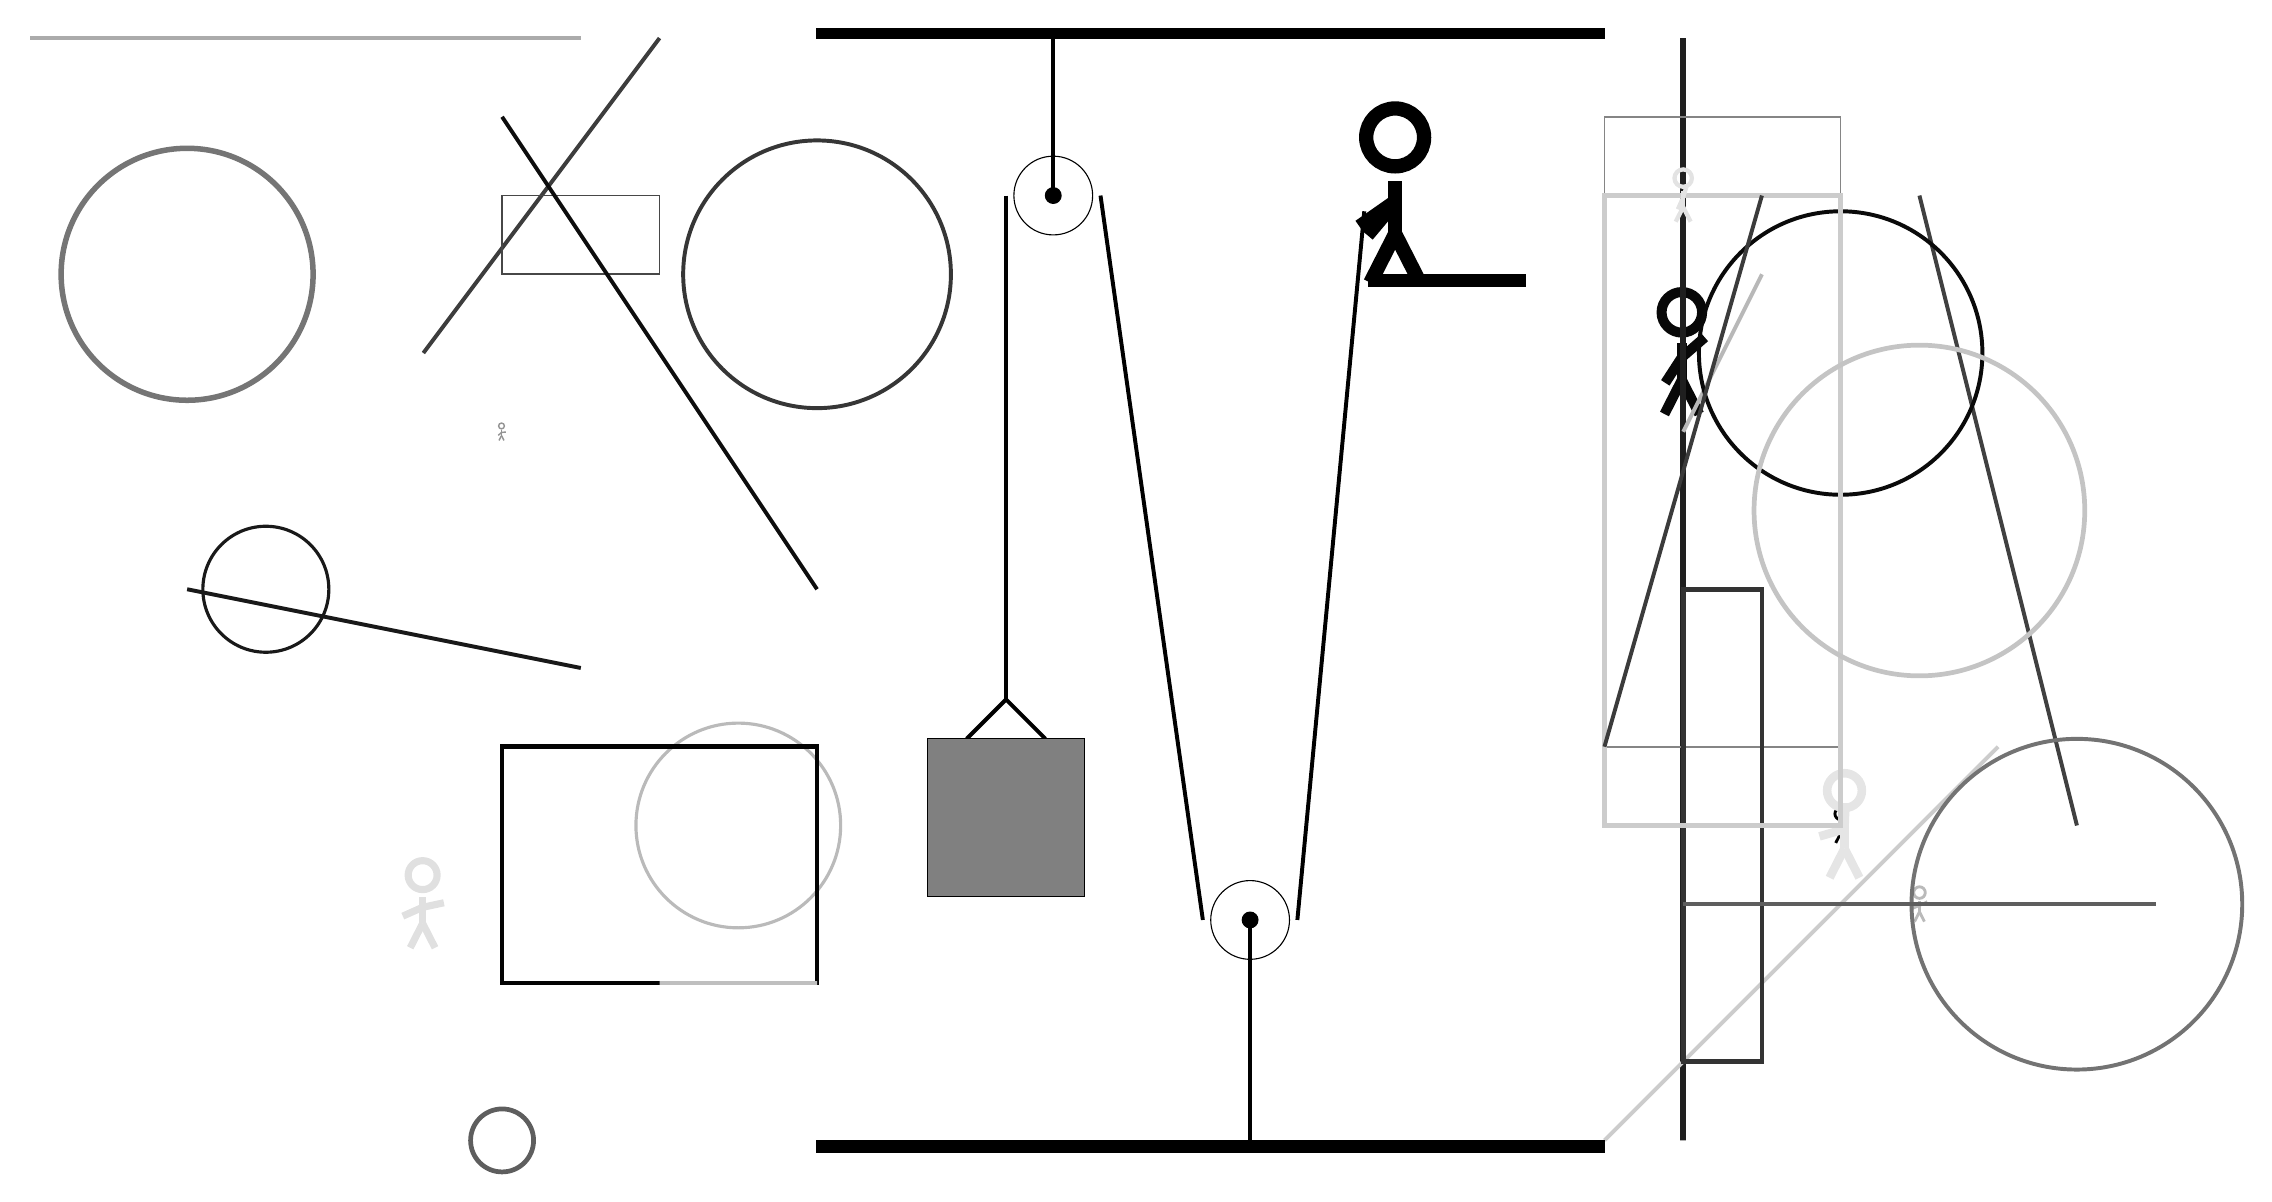
\begin{tikzpicture}
			%%%%% START %%%%%
			
			\draw[fill=black] (-2, 14) rectangle (8, 14.125);
			
			\node[line width=0.3mm, color=black!42] at (-6, 9) {\Strichmaxerl[1][43][4]};
			
			\draw[line width=0.5mm, color=black!90](-5, 6) -- (-10, 7);
			\node[line width=0.5mm, color=black!100] at (11, 4) {\Strichmaxerl[2][39][40]};
			\node[line width=0.2mm, color=black!97] at (9, 10) {\Strichmaxerl[7][57][41]};
			
			\draw [line width=0.2mm, color=black!32](14, 1) circle (0.0);
			\draw[line width=0.7mm, color=black!88] (9, 0) rectangle (9, 14);
			
			\draw[line width=0.5mm, color=black!33](-5, 14) -- (-12, 14);
			\draw[line width=0.5mm, color=black!28](9, 9) -- (10, 11);
			\draw [line width=0.4mm, color=black!27](-3, 4) circle (1.3);
			\node[line width=0.3mm, color=black!27] at (12, 3) {\Strichmaxerl[2][22][25]};
			
			\draw [line width=0.4mm, color=black!90](-9, 7) circle (0.8);
			\draw [line width=0.6mm, color=black!63](-6, 0) circle (0.4);
			\draw[line width=0.2mm, color=black!48] (8, 5) rectangle (11, 13);
			
			\draw[line width=0.5mm, color=black!20](13, 5) -- (8, 0);
			\draw[line width=0.6mm, color=black!80] (10, 7) rectangle (9, 1);
			\draw [line width=0.7mm, color=black!54](-10, 11) circle (1.6);
			
			\node[line width=0.3mm, color=black!10] at (11, 4) {\Strichmaxerl[6][16][88]};
			\draw[line width=0.6mm, color=black!99] (-2, 2) rectangle (-6, 5);
			\draw[line width=0.5mm, color=black!75](12, 12) -- (14, 4);
			\draw [line width=0.5mm, color=black!79](-2, 11) circle (1.7);
			\draw [line width=0.5mm, color=black!96](11, 10) circle (1.8);
			\draw[line width=0.6mm, color=black!20] (8, 12) rectangle (11, 4);
			
			\node[line width=0.3mm, color=black!12] at (-7, 3) {\Strichmaxerl[5][24][12]};
			\draw [line width=0.5mm, color=black!55](14, 3) circle (2.1);
			\draw[line width=0.5mm, color=black!76](-7, 10) -- (-4, 14);
			
			\draw[line width=0.5mm, color=black!77](8, 5) -- (10, 12);
			\draw [line width=0.6mm, color=black!23](12, 8) circle (2.1);
			\draw[line width=0.5mm, color=black!63](9, 3) -- (15, 3);
			\draw[line width=0.4mm, color=black!25] (-4, 2) rectangle (-2, 2);
			\draw[line width=0.2mm, color=black!72] (-4, 11) rectangle (-6, 12);
			\draw[line width=0.5mm, color=black!95](-6, 13) -- (-2, 7);
			
			\node[line width=0.5mm, color=black!11] at (9, 12) {\Strichmaxerl[3][66][73]};
			
			\draw (3.5, 2.8) circle (0.5);
			\draw[fill=black] (3.5, 2.8) circle (0.1);
			\draw[line width=0.5mm] (3.5, 2.8) -- (3.5, 0);
			
			\draw (1, 12) circle (0.5);
			\draw[fill=black] (1, 12) circle (0.1);
			\draw[line width=0.5mm] (1, 14) -- (1, 12);
			
			\draw[line width=0.5mm](-0.1, 5.1) --  (0.4, 5.6) -- (0.9, 5.1);
			\draw[fill=black!50] (-0.6, 5.1) rectangle (1.4, 3.1);
			
			\draw[line width=0.5mm](0.4, 12) -- (0.4, 5.6);
			\centerarc[line width=0.5mm](1, 12)(180:0:0.6)
			\draw[line width=0.5mm](1.6, 12) -- (2.9, 2.8);
			\centerarc[line width=0.5mm](3.5, 2.8)(180:360:0.6)
			\draw[line width=0.5mm](4.1, 2.8) -- (4.95, 11.8);
			
			\node at (5.3, 12) {\Strichmaxerl[10][35][-130]};
			\draw[fill=black] (5, 11) rectangle (7, 10.85);
			
			\draw[fill=black] (-2, 0) rectangle (8, -0.15);
			
			%%%%% END %%%%%
		\end{tikzpicture}
	\end{figure}	
\end{document}